 \thispagestyle{cackithitoannone}
\pagestyle{cackithitoan}
\everymath{\color{cackithi}}
\graphicspath{{../cackithi/pic/}}
\blfootnote{{\color[named]{cackithi}$^1$Trường THPT chuyên Khoa học Tự nhiên, Đại học KHTN, Đại học Quốc gia Hà Nội.}}
\begingroup
\AddToShipoutPicture*{\put(0,616){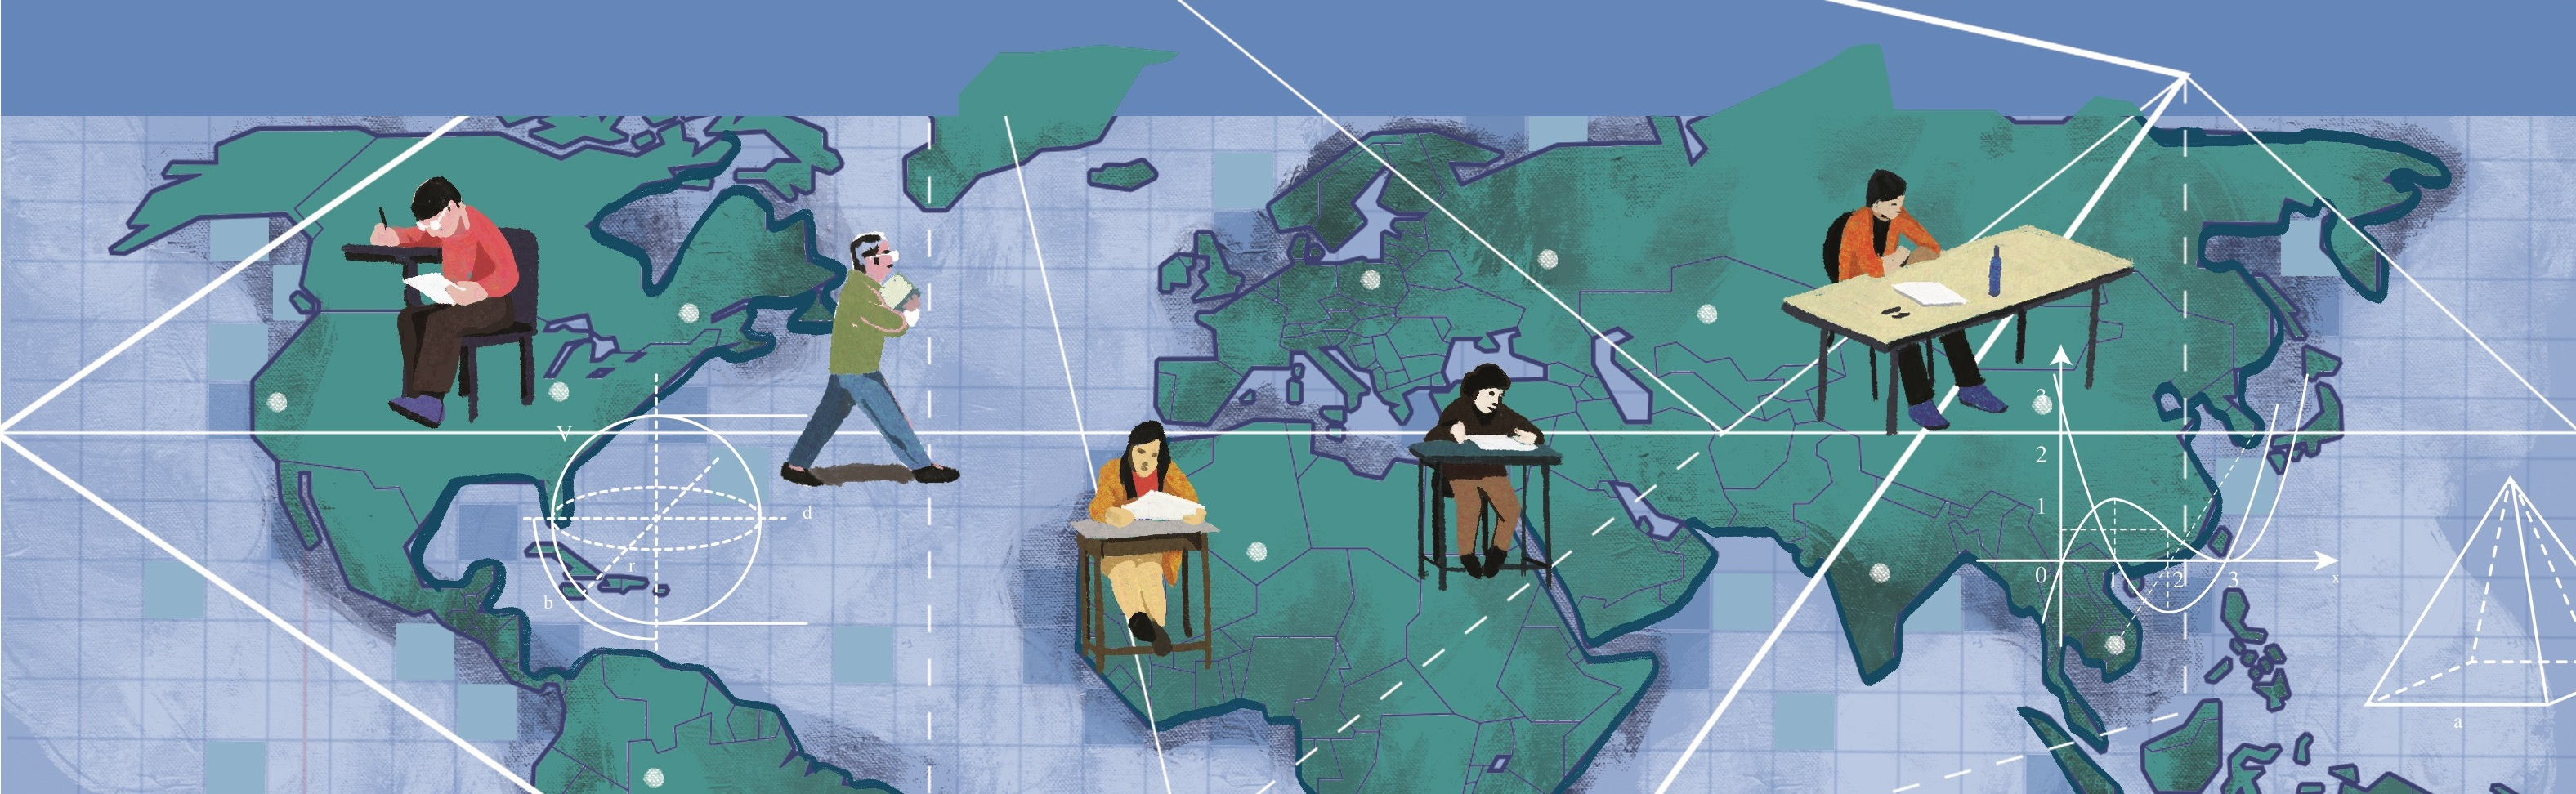
\includegraphics[width=19.3cm]{../bannercackithi}}} 
\AddToShipoutPicture*{\put(98,522){
\includegraphics[scale=1]{../tieude2.pdf}}} 
\centering
\endgroup
\vspace*{192pt}

\begin{tBox}
	Tại kỳ thi Olympic Toán quốc tế lần thứ $63$, diễn ra từ ngày $6/7/2022$ đến ngày $16/7/2022$ tại Oslo, Na Uy, đội tuyển Việt Nam, đã đạt thành tích xuất sắc, giành được $2$ HCV, $2$ HCB và $2$ HCĐ:
	\begin{itemize}[leftmargin = 10pt, itemsep =0.5pt, parsep =0.5pt, topsep =0.5pt]
		\item Ngô Quý Đăng, lớp $12$, trường THPT chuyên KHTN, ĐH KHTN, ĐHQG Hà Nội, $42$ điểm, HCV.
		\item Phạm Việt Hưng, lớp $11$, trường THPT chuyên KHTN, ĐH KHTN, ĐHQG HÀ Nội, $39$ điểm, HCV.
		\item Phạm Hoàng Sơn, lớp $12$, trường PTNK, ĐHQG Tp HCM, $30$ điểm, HCB.
		\item Nguyễn Đại Dương, lớp $12$, trường THPT chuyên Lam Sơn, Thanh Hóa, $29$ điểm, HCB.
		\item Vũ Ngọc Bình, lớp $12$, THPT chuyên Vĩnh Phúc, $28$ điểm, HCĐ.
		\item Hoàng Tiến Nguyên, lớp $12$, THPT chuyên Phan Bội Châu, Nghệ An, $28$ điểm, HCĐ.
	\end{itemize}
	Tạp chí Pi xin chúc mừng các em!
\end{tBox}

\begin{multicols}{2}
	Bài viết này là những ghi chép của cá nhân tác giả (dưới tư cách là quan sát viên $C$) về chuyến đi cùng đoàn Việt Nam dự thi Olympic Toán quốc tế năm $2022$ ở Na Uy.
	\vskip 0.05cm
	{\bf\color{cackithi}Một vài ghi chép về kỳ thi}
	\vskip 0.05cm
	Lần đầu tiên đến một nước Bắc Âu, tôi có cảm giác vui pha chút lo lắng. Vui vì sắp đến một đất nước được coi là quốc gia giàu có của châu Âu, nước có mức sống thuộc hàng cao nhất châu Âu (GDP bình quân đầu người cao thứ hai trong số các quốc gia châu Âu). Tham gia đoàn đưa học sinh đi thi Olympic Toán quốc tế, tôi không lo lắng sao được. Cùng chung cảm giác với các thành viên khác, liệu đoàn Việt Nam mình có được kết quả tốt hay không? Riêng tôi, với tư cách là giáo viên trường THPT chuyên KHTN, trường có hai em học sinh trong đoàn là Ngô Quý Đăng (lớp $12$) và Phạm Việt Hưng (lớp $11$) đi thi, tôi mong rằng các em học sinh của trường mình sẽ có thành tích tốt nhất. Cảm giác hồi hộp ấy cứ theo tôi hàng ngày, và rồi cũng vơi dần khi khám phá nhiều điều thú vị ở Oslo.
	\vskip 0.05cm
	Đoàn chúng tôi đi từ Hà Nội trên máy bay của hãng hàng không Vietnam Airlines, quá cảnh qua Paris và tới Na Uy trên máy bay của hãng Scandinavi. Máy bay của họ nhỏ hơn máy bay của mình, sau hơn $2$ tiếng đống hồ chúng tôi đã bay trên bầu trời Na Uy. Ngay từ trên máy bay, tôi đã thấy Thủ đô Oslo xinh đẹp hiện dần ra. Đất nước Na Uy có rất nhiều hồ. Tầm $14$h, giờ máy bay hạ cánh xuống sân bay quốc tế Gardermoen của Oslo.
	\begin{figure}[H]
		\vspace*{-5pt}
		\centering
		\captionsetup{labelformat= empty, justification=centering}
		\includegraphics[width= 1\linewidth]{figure8108}
		\caption{\small\textit{\color{cackithi}Ảnh chụp một góc Oslo từ trên máy bay.}}
		\vspace*{-10pt}
	\end{figure}
	Ngay ở sân bay ban tổ chức đã tiếp đón đoàn rất chu đáo và hướng dẫn rất chi tiết. Tôi đã được nghe nói trong mùa hè, ngày sẽ dài hơn đêm, nhất là ở vùng này, thời gian hè còn có cả những đêm trắng. Quả đúng thế, dù $12$ giờ đêm mà bầu trời có vẻ mới chập tối, còn $4$ giờ thì trời đã hửng sáng. Dù đang giữa hè nhưng thời tiết ở đây khá lạnh, cho cảm giác như mùa đông của Hà Nội vậy. Cũng may là mọi thành viên của đoàn đều đã được biết điều này từ trước nên ai cũng đều có áo ấm phù hợp. Có một sự cố nhỏ là trong đoàn có một em học sinh bị thất lạc hành lý. Chờ ít lâu ở sân bay để xử lý điều đó rồi chúng tôi cũng được đưa về khách sạn, nơi sẽ diễn ra kỳ thi Olympic Toán quốc tế $2022$. Các đoàn khác cũng tề tựu cả về đây. Khách sạn rất lớn, với vẻ bên ngoài khá choáng ngợp. Với rất nhiều đoàn tham gia (kỳ thi năm nay có hơn $100$ nước tham dự) nên sự đông vui, náo nhiệt bên trong khuôn viên khiến cho bạn cảm thấy như thế giới được thu nhỏ bên trong khách sạn này vậy. 
	\vskip 0.05cm
	Ngày tiếp theo, trưởng đoàn là GS. Lê Anh Vinh đã bị ``nhốt" để chuẩn bị đề thi, còn và phó đoàn là TS. Lê Bá Khánh Trình ở ngoài (khu vực cách ly) thì rất cẩn thận, luôn quan tâm dặn dò các em học sinh và các quan sát viên chúng tôi. Tranh thủ trước khi ăn sáng, chúng tôi ngó qua quang cảnh khu vực nơi mình nghỉ ngơi. Bên ngoài, phố xá yên bình quá, các đoàn tàu điện qua lại, hành khách lên xuống bình lặng, không ồn ào nhộn nhịp xe cộ (mà có phần lộn xộn) như ở Hà Nội. Những chậu hoa nhiều màu sắc tô điểm thêm cho các góc phố thêm xinh tươi, thanh bình. Quen dần với không khí khô mát, dù có hơi lạnh, chúng tôi lại thấy khí hậu buổi sáng Oslo rất tuyệt vời. 
	\begin{figure}[H]
		\vspace*{-5pt}
		\centering
		\captionsetup{labelformat= empty, justification=centering}
		\includegraphics[width= 1\linewidth]{figure8109}
		\caption{\small\textit{\color{cackithi}Ảnh tác giả chụp bên ngoài khách sạn đoàn nghỉ~chân.}}
		\vspace*{-10pt}
	\end{figure}
	Đã đến $14$h chiều và Ban tổ chức tiến hành lễ khai mạc. Không khí rất trang trọng. Ai nấy đều ngóng lên sân khấu chờ xem đoàn nước mình hiện ra. Cuối cùng thì đoàn học sinh của Việt Nam xuất hiện với lá cờ đỏ sao vàng trên sân khấu. Tự hào quá! 
	\vskip 0.05cm
	Trên phông nền hình ảnh của buổi lễ khai mạc, Ban tổ chức giới thiệu rất nhiều về đất nước và con người Na Uy. Tuy vậy ấn tượng nhất với tôi từ những ngày còn đi học đó là nhà toán học Na Uy Niels Henrik Abel. Phải nói thêm, ông là thần tượng của tôi. Ông sinh ngày $05$ tháng $8$ năm $1802$ tại  Nedstrand (Na Uy), và mất ngày $16$ tháng $4$ năm $1829$ tại Froland (Na Uy). Tôi đã mong ước có ngày được đến trước tượng đài Abel ở Oslo. Ngày hôm nay, ước mơ đó đã thành sự thật: tôi đã được đặt chân tới quê hương của Abel! 
	\vskip 0.05cm
	Ngày hôm sau, các em học sinh bước luôn vào kỳ thi. Chắc rằng không khí bên trong phòng thi cũng khá căng thẳng. Còn ở bên ngoài, chúng tôi ai cũng thầm mong các em sẽ giải được các bài toán khó. Tin tưởng vào các em nên chúng tôi cũng giảm bớt lo lắng. 
	\vskip 0.05cm
	Ngày thi đầu tiên, khi các em đi về, thầy Trình và chúng tôi đều cố gắng tạo tâm lý thoải mái nhất cho các em, không hỏi han nhiều các em về kết quả ngày $1$. Riêng với tôi thì khi xem đề thi ngày $1$ ở trên mạng, tôi cũng thầm lo lắng vì ngày $1$ không hề có môn hình học, vốn là thế mạnh của đoàn Việt Nam.
	\vskip 0.05cm
%	\begin{figure}[H]
%		\vspace*{-5pt}
%		\centering
%		\captionsetup{labelformat= empty, justification=centering}
%		\includegraphics[width= 1\linewidth]{figure8111}
%		\caption{\small\textit{\color{cackithi}Tác giả đặt hoa ở tượng đài nhà Toán học Niels Henrik Abel.}}
%		\vspace*{-10pt}
%	\end{figure}
	Sang ngày thi thứ hai, sau khi ăn sáng, xe buýt đón các em đi thi. Như ngày thi đầu, chúng tôi đưa các em ra xe và các em đi cùng thầy Trình tới địa điểm thi. Sau đó, tôi tranh thủ đi mua hoa để viếng thăm tượng đài Abel. May mắn là tôi đã nhanh chóng tìm được một tiệm hoa tươi và mua được $10$ bông hoa hồng đỏ thắm. Bản đồ Google đã chỉ đường cho tôi tới tượng đài Abel. Hóa ra tượng đài rất gần cung điện Hoàng gia Na Uy, là nơi tôi đã có dịp ghé thăm hôm trước, khi các em làm bài thi ngày đầu tiên.
	\vskip 0.05cm
	Tôi được biết về Abel từ khi học lớp $7$ qua những cuốn tư liệu, lịch sử toán học, và một cuốn truyện viết về ông. Từ ngày đó, tuy rất thích ông nhưng tôi chỉ thấy ``lạ" là tại sao ông mất khi còn quá trẻ ($27$ tuổi). Rồi qua những ngày học đại học, khi được học qua nhiều khái niệm và định lý mang tên ông, tôi lại mày mò đọc về ông nhiều hơn (cả bằng tiếng Anh) ở trên mạng. Lúc đó, tôi mới thấy thêm nhiều điều kỳ diệu về ông. Dường như những tư tưởng toán học của ông đã đi trước thời đại của ông nhiều năm. Sự say mê Toán của Abel đã vượt qua nhiều giới hạn thời đó. Nhưng không may thay, tư tưởng của ông không được những nhà toán đọc đương đại lúc đó nhìn nhận và đánh giá một cách công bằng (trừ một vài người bạn thân của ông như Jacobi và Crelle). Sau chuyến công du châu Âu không thu được mấy kết quả, ông lại về Oslo, vẫn mang trong mình sự đam mê cháy bỏng với Toán, nhưng bên cạnh là một cuộc sống đầy vất vả. Ông vẫn phải duy trì cuộc sống bằng công việc dạy học. Có lẽ vì sự đam mê quá lớn của ông với Toán, ông vẫn làm Toán và trăn trở với Toán. Đến một thời điểm sức khỏe suy kiệt, ông bị nhiễm bệnh lao và ra đi ở tuổi $27$. Câu chuyện về sự đam mê Toán và sự ra đi quá sớm của ông đã khiến những người yêu Toán thời sau không khỏi xót thương. Hậu thế sau này đã trả lại sự công bằng và nhìn nhận ông như là một trong những nhà Toán học vĩ đại nhất thời điểm đó. Viện hàn lâm Khoa học Na Uy đã dành một giải thưởng mang tên ông, được coi là một trong những giải thưởng danh giá nhất trong Toán học, để vinh danh những nhà Toán học có những thành tựu xuất sắc nhất. Nhưng tiếc thay, ông không còn sống để thấy được những vinh dự đó. Đặt đóa hoa hồng tươi thắm bên cạnh tượng đài để tưởng nhớ đến Abel, tôi thấy xúc động và ngậm~ngùi!
	\begin{figure}[H]
		\vspace*{-5pt}
		\centering
		\captionsetup{labelformat= empty, justification=centering}
		\includegraphics[width= 1\linewidth]{figure8110}
		\caption{\small\textit{\color{cackithi}Đoàn sáu học sinh Việt Nam xuất hiện với cờ đỏ sao vàng ở lễ khai mạc.}}
		\vspace*{-10pt}
	\end{figure}
	Kết thúc hai ngày thi, chúng tôi cũng không hỏi han các em quá nhiều về bài làm, để các em thoải mái giao lưu với các bạn và tham quan Oslo. Tuy vậy, nghe qua Hưng và Đăng nói làm trọn vẹn $6$ bài, tôi khá vui nhưng cũng xen lẫn tò mò. Không lẽ IMO với hai em ``dễ" vậy, làm trọn vẹn nhẹ như không!
	\vskip 0.05cm
	Trong những ngày sau đó, cả đoàn hồi hộp đợi thầy Vinh và thầy Trình chấm thi. Thỉnh thoảng, các anh em trong đoàn chúng tôi lại rủ nhau đi thăm phố xá, chụp một vài cảnh đẹp lưu giữ kỷ niệm về Oslo và giới thiệu với mọi người biết thêm về một thành phố yên bình: tòa thị chính Thành phố, nơi trao giải Nobel hòa bình, những tượng đài, những chú bồ câu nhẩn nha tản bộ như cùng mọi người trên hè phố và những tòa nhà dọc theo phố phường (không cao lắm như các tòa nhà mới mọc lên ở Thủ đô nước ta). Chúng tôi cũng thường đi dọc bờ sông (hay là ra cảng Oslo) ngắm bầu trời cao lồng lộng, trong xanh với những đám mây trắng như bông bồng bềnh, làm tăng vẻ đẹp quyến rũ của Oslo.
	\vskip 0.05cm
	Sau khi có kết quả thi thì tôi không khỏi không vui mừng cho thành tích chung của đoàn và đặc biệt là của hai em học sinh từ THPT chuyên KHTN. Thầy hiệu trưởng Lê Công Lợi đã gọi cho tôi nhiều lần trong khi kỳ thi diễn ra. Tới khi có kết quả chính thức thì cả trường đều rất vui.
	\begin{figure}[H]
		\vspace*{-5pt}
		\centering
		\captionsetup{labelformat= empty, justification=centering}
		\includegraphics[width= 1\linewidth]{figure8112}
		\caption{\small\textit{\color{cackithi}Đoàn Việt Nam và đoàn Thái Lan chụp lưu niệm ở bên ngoài tòa thị chính, nơi diễn ra lễ trao huy chương IMO.}}
		\vspace*{-10pt}
	\end{figure}
	Thời gian $10$ ngày ở Na Uy nhanh chóng trôi qua.  Kết quả cuộc thi Olympic toán quốc tế năm $2022$ (IMO $2022$) chính thức công bố vào ngày $15/7$. Đây là một kết quả ngoài sức mong đợi của nhiều người: đoàn Việt Nam đứng thứ $4$ trong tổng số $104$ quốc gia, vùng lãnh thổ tham dự, và cả sáu thí sinh đoàn Việt Nam đều đoạt huy chương (gồm hai Vàng, hai Bạc và hai Đồng). Hai học sinh của trường THPT chuyên Khoa học tự nhiên (ĐH Quốc gia Hà Nội) đều đạt huy chương vàng. Đặc biệt, em Ngô Quý Đăng là một trong những thí sinh đạt điểm tuyệt đối $42/42$. Tuy thành công như vậy nhưng trong lòng chúng tôi vẫn còn có xen lẫn khá nhiều tiếc nuối khi điểm xét giải  chưa được như mong đợi của chúng tôi. Nhưng đúng là cuộc chơi nào thì cũng đều có nụ cười và nước mắt, chúng tôi và các em đều hiểu điều đó. Thế nên sau đó nửa ngày là các em lại chơi vui vẻ như mới bắt đầu kỳ thi.
	\vskip 0.05cm
	Sau lễ trao giải, cả đoàn ở Oslo thêm một ngày rồi ra sân bay về nước. Đoàn chúng tôi quá cảnh qua sân bay Frankfurt của Đức. Ở đây khi chuyển sang máy bay của Vietnam Airlines, ai cũng mừng như thấy người nhà. Có lẽ vì đã xa Việt Nam $10$ ngày nên ai cũng nhớ nhà. Sau hành trình bay $12$h, chúng tôi hạ cánh xuống sân bay quốc tế Nội Bài, kết thúc một chuyến đi thành công tốt đẹp.
	\vskip 0.05cm
	Tôi xin được nói lời cảm ơn và tri ân tới thầy Lê Anh Vinh và thầy Lê Bá Khánh Trình, hai người thầy lớn đã bền bỉ làm trưởng phó đoàn Việt Nam hơn $10$ năm qua, mang lại thêm nhiều thành tích to lớn cho đoàn IMO của Việt Nam. Cá nhân tôi xin nói lời cảm ơn sâu sắc thầy Nguyễn Vũ Lương, kiến trúc sư trưởng của đội tuyển toán THPT chuyên KHTN, người đã kiến tạo những thành công cho đội tuyển Toán của trường THPT chuyên KHTN nhiều năm qua.
	\vskip 0.05cm
	{\bf\color{cackithi}Về bài toán hình học duy nhất của kỳ thi}
	\vskip 0.05cm 
	Kỳ thi IMO năm $2022$ có duy nhất một bài toán hình học, nằm ở vị trí bài toán đầu tiên của ngày thi thứ hai. Mặc dù được coi là bài toán dễ nhất trong ngày thi thứ $2$, nhưng tôi đánh giá đó là một bài toán hay và có giá trị. Ngay sau ngày thi thứ $2$, tôi cũng đã có một vài ý phát triển và thảo luận về bài toán này ở [$1$]. Tôi xin chia sẻ lại cùng bạn đọc nội dung bài toán tổng quát đó cùng với lời giải của mình (tham khảo [$1$]).
	\vskip 0.05cm
	\textbf{\color{cackithi}Bài toán} (Một tổng quát hóa cho bài $4$ của Đề thi IMO $2022$) Cho ngũ giác lồi $ABCDE$ và các điểm $M$ và $N$ nằm trong $ABCDE$ sao cho tứ giác $CDMN$ nội tiếp, $\triangle MBD$ đồng dạng với $\triangle NEC$ và $\angle ABD=\angle AEC$. Đường thẳng $AB$ lần lượt cắt các đường thẳng $CD$ và $CM$ tại các điểm $P$ và $Q$ (ta có thể giả sử $P$, $B$, $A$, $Q$ nằm trên đường thẳng theo thứ tự đó). Đường thẳng $AE$ lần lượt cắt các đường thẳng $CD$ và $DN$ tại hai điểm $R$ và $S$ (ta có thể giả sử rằng $R$, $E$, $A$, $S$ nằm trên đường thẳng theo thứ tự đó). Chứng minh rằng các điểm $P$, $S$, $Q$, $R$ cùng nằm trên một đường tròn.
	\begin{figure}[H]
		\vspace*{-5pt}
		\centering
		\captionsetup{labelformat= empty, justification=centering}
		\includegraphics[width= 0.7\linewidth]{figure8082}
		\caption{\small\textit{\color{cackithi}Lời giải cho bài toán tổng quát.}}
		\vspace*{-10pt}
	\end{figure}
	\setlength{\abovedisplayskip}{6pt}
	\setlength{\belowdisplayskip}{6pt}
	\textbf{\color{cackithi}Lời giải.} Gọi $J$ là giao điểm của $DN$ và $CM$. Từ $\triangle MBD\sim\triangle NEC$ ta suy ra $\angle MBD=\angle NEC$. Kết hợp với $\angle ABD=\angle AEC$ ta thu được 
		\begin{align*}\angle ABM=\angle AEN.\tag{$1$}\end{align*}
		Cũng từ $\angle BMD=\angle CNE$ và $\angle CMD=\angle DNC$ (vì tứ giác $CDMN$ nội tiếp), ta suy ra
		\begin{align*}
			\angle BMC=\angle END
		\end{align*} hay là 
		\begin{align*}
			\angle BMQ=\angle ENS. \tag{$2$}
		\end{align*}
		Từ ($1$) và ($2$) ta thu được $\triangle NES\sim\triangle MBQ$. Vì vậy ta có 
		\begin{align*}
			\frac{QM}{NS}=\frac{BM}{NE}=\frac{DM}{CN}=\frac{JM}{JN},
		\end{align*}
		dẫn đến
		\begin{align*}
			\frac{JM}{MQ}=\frac{JN}{NS}.
		\end{align*}
		Vậy theo định lý Thales đảo, ta suy ra \linebreak$MN\parallel SQ$. Từ đây,
		\begin{align*}
			\angle SQM=\angle NMC=\angle NDC,
		\end{align*} hay tứ giác $SQDC$ nội tiếp. Ta tiếp tục có biến đổi góc như sau
		\begin{align*}
			\angle QSR&=\angle QSD-\angle RSD\\
			&=\angle QCD-\angle PQC=\angle QPR,
		\end{align*}
		hay $SQRP$ nội tiếp. Ta hoàn thành lời giải.
	\vskip 0.05cm
	{\bf\color{cackithi}Đôi lời bàn:}
	Hình học phẳng thường được coi là thế mạnh của đoàn Việt Nam. Như với bài $4$ của đề thi này thì cả $6$ thí sinh đoàn Việt Nam đều được điểm tối đa. Tuy vậy, vì là thế mạnh nên nếu bài hình là bài toán khó hơn thì theo chủ quan của tôi còn đem lại chút lợi thế hơn nữa cho đội tuyển Việt Nam. Tôi cũng thường tham gia tập huấn cho đội tuyển Việt Nam thi IMO về phần hình học trong $10$ năm gần đây. Theo ý chủ quan của tôi thì các học sinh của của chúng ta không hề sợ bài hình ``khó", nhưng lại hay va vấp ở những bài hình ``đẹp". Nếu bài hình ``đẹp" mà rơi vào những bài toán cuối của mỗi đề thi (được coi là những bài khó nhất) thì sẽ rất thách thức cho các học sinh của chúng ta, mặc dù hình học vẫn là thế mạnh của đoàn Việt Nam. Vì điều trăn trở này nên trong công việc tập huấn, tôi luôn cố gắng tìm những bài toán ``đẹp" có nhiều thách thức, phù hợp với kỳ thi IMO, cho các em thay vì những bài toán rối rắm, mang nặng tính kỹ thuật, có thể được hỗ trợ nhiều bằng máy tính. Tôi cũng mong rằng những bài toán đẹp nhưng vẫn có nhiều tính thách thức sẽ xuất hiện nhiều hơn trong các kỳ thi của Việt Nam.
	\vskip 0.05cm
	\textbf{\color{cackithi}Tài liệu tham khảo}
	\vskip 0.05cm
	[$1$] \url{https://artofproblemsolving.com/com} \url{munity/c6h2883216p25635154}.
\end{multicols}
\newpage
\begingroup
\AddToShipoutPicture*{\put(148,700){
\includegraphics[scale=1]{../tieude1.pdf}}} 
\centering
\endgroup
\vspace*{5pt}

\begin{multicols}{2}
	Trong phần đầu chuyên mục, chúng tôi sẽ trình bày lời giải của các bài toán trong kỳ thi Olympic Toán Liên bang Nga năm học $2021-2022$ đăng trong số báo $5/2022$. 
	\begin{figure}[H]
		\vspace*{-5pt}
		\centering
		\captionsetup{labelformat= empty, justification=centering}
		
\includegraphics[width= 1\linewidth]{gocolympic}
		\vspace*{-15pt}
	\end{figure}
	{\bf\color{cackithi} OC$\pmb{10.}$}(Lớp $6$) Ở một đất nước có những con rồng sinh sống, mỗi con có một trong ba màu: đỏ, xanh lá cây hoặc xanh lam. Mỗi con rồng có ba đầu, mỗi cái đầu luôn nói thật hoặc luôn nói dối. Hơn nữa, mỗi con rồng đều có ít nhất một cái đầu luôn nói thật. 
	Một hôm, $530$ con rồng ngồi quanh một bàn tròn và các đầu của mỗi con đều nói:
	\vskip 0.1cm
	$\bullet$ Đầu thứ nhất: ``Ngồi sát bên trái tôi là một con rồng xanh lá cây."
	\vskip 0.1cm
	$\bullet$ Đầu thứ hai: ``Ngồi sát bên phải tôi là một con rồng xanh lam."
	\vskip 0.1cm
	$\bullet$ Đầu thứ ba: ``Không có con rồng đỏ nào ngồi cạnh tôi."
	\vskip 0.1cm
	Hỏi có thể có nhiều nhất bao nhiêu con rồng đỏ ngồi trong bàn?
	\vskip 0.1cm
	\textit{Lời giải.} Giả sử $A$ là một con rồng đỏ bất kỳ. Ta nhận xét rằng con rồng ngồi sát bên trái của $A$ có đầu thứ hai và ba nói dối, do đó đầu thứ nhất phải nói thật. Như vậy ngồi sát bên trái của con rồng này là một con rồng xanh lá cây, giả sử là $B.$ Lý luận tương tự, ta thấy cũng có một con rồng $C$ màu xanh lam ngồi bên phải $A$ và cách $A$ một vị trí.
	\vskip 0.1cm
	Như vậy, với mỗi con rồng đỏ $A,$ ta tìm được một bộ ba con rồng ngồi cách nhau 1 vị trí theo chiều kim đồng hồ là $C, A, B$ và có màu tương ứng là xanh lam, đỏ, xanh lá cây. Dễ nhận thấy không có con rồng nào thuộc hai bộ ba khác nhau. Do đó nếu $k$ là số rồng đỏ thì $3k\le 530,$ tức là $k\le 176.$
	\vskip 0.1cm
	Giá trị lớn nhất này đạt được khi ta có hai con rồng xanh lam và xanh lá cây ở $175$ khoảng giữa của $176$ con rồng đỏ, riêng một khoảng giữa xếp $4$ con rồng xanh lam và xanh lá cây (xem hình vẽ).
	\begin{figure}[H]
		\vspace*{-5pt}
		\centering
		\captionsetup{labelformat= empty, justification=centering}
		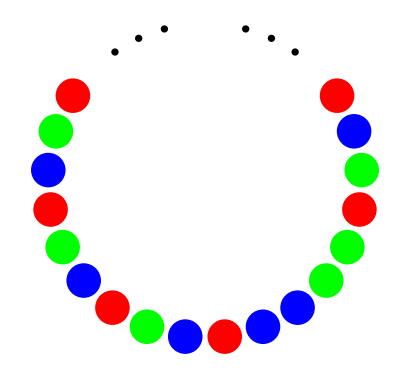
\includegraphics[width= 1\linewidth]{OC10}
		\vspace*{-15pt}
	\end{figure}
	{\bf\color{cackithi} OC$\pmb{11.}$} Người ta cắt một dải hình chữ nhật có chiều dài $16$ thành hai dải dài $9$ và $7$. Hai dải này được đặt trên bàn như hình vẽ bên. Biết rằng diện tích của phần chỉ bị che phủ bởi dải bên trái là $27$ và diện tích của phần chỉ bị che phủ bởi dải bên phải là $18$. Tìm diện tích của phần được che phủ bởi cả hai dải.
	\begin{figure}[H]
		\vspace*{-10pt}
		\centering
		\captionsetup{labelformat= empty, justification=centering}
		\begin{tikzpicture}[scale=0.7]
			\draw[cackithi] (0,0) rectangle (4.5,2.2);
			\draw[cackithi] (1.85,0) -- (1.85,2.2);
			\draw[cackithi] (3.3,0) -- (3.3,2.2);
			\node at (0.925,1.1){$27$};
			\node at (2.575,1.1){$?$};
			\node at (3.9,1.1){$18$};
			
			\draw [decorate,
			decoration = {calligraphic brace}] (0,2.3) --  (3.3,2.3) node[above, midway] {$9$};
			
			\draw [decorate,
			decoration = {calligraphic brace, mirror}] (1.85,-0.1) --  (4.5,-0.1) node[below, midway] {$7$};
		\end{tikzpicture}
		\vspace*{-15pt}
	\end{figure}
	\textit{Lời giải.} Vì hai dải băng đều là các hình chữ nhật có một cạnh bằng nhau nên tỷ lệ diện tích giữa giải băng bên trái và dải băng bên phải là $\dfrac{9}{7}.$ Gọi $S$ là diện tích 
	phần bị che phủ bởi cả hai dải băng, ta có
	\begin{align*}
		\frac{27+S}{18+S}=\frac{9}{7}.
	\end{align*}
	Từ đó ta tìm được $S=13{,}5$.
	\vskip 0.1cm
	\textit{\color{cackithi}OC$\pmb{12.}$}(Lớp $7$) Có bảy hộp xếp quanh một vòng tròn, mỗi hộp chứa một số đồng xu.
	Hình bên dưới cho biết có bao nhiêu đồng xu trong mỗi hộp.
	\vskip 0.1cm
	Mỗi lần, ta được phép di chuyển một đồng xu sang một trong hai hộp liền kề. Hỏi cần di chuyển ít nhất bao nhiêu lần để số đồng xu trong tất cả các hộp bằng nhau?
	\begin{figure}[H]
		\vspace*{-5pt}
		\centering
		\captionsetup{labelformat= empty, justification=centering}
		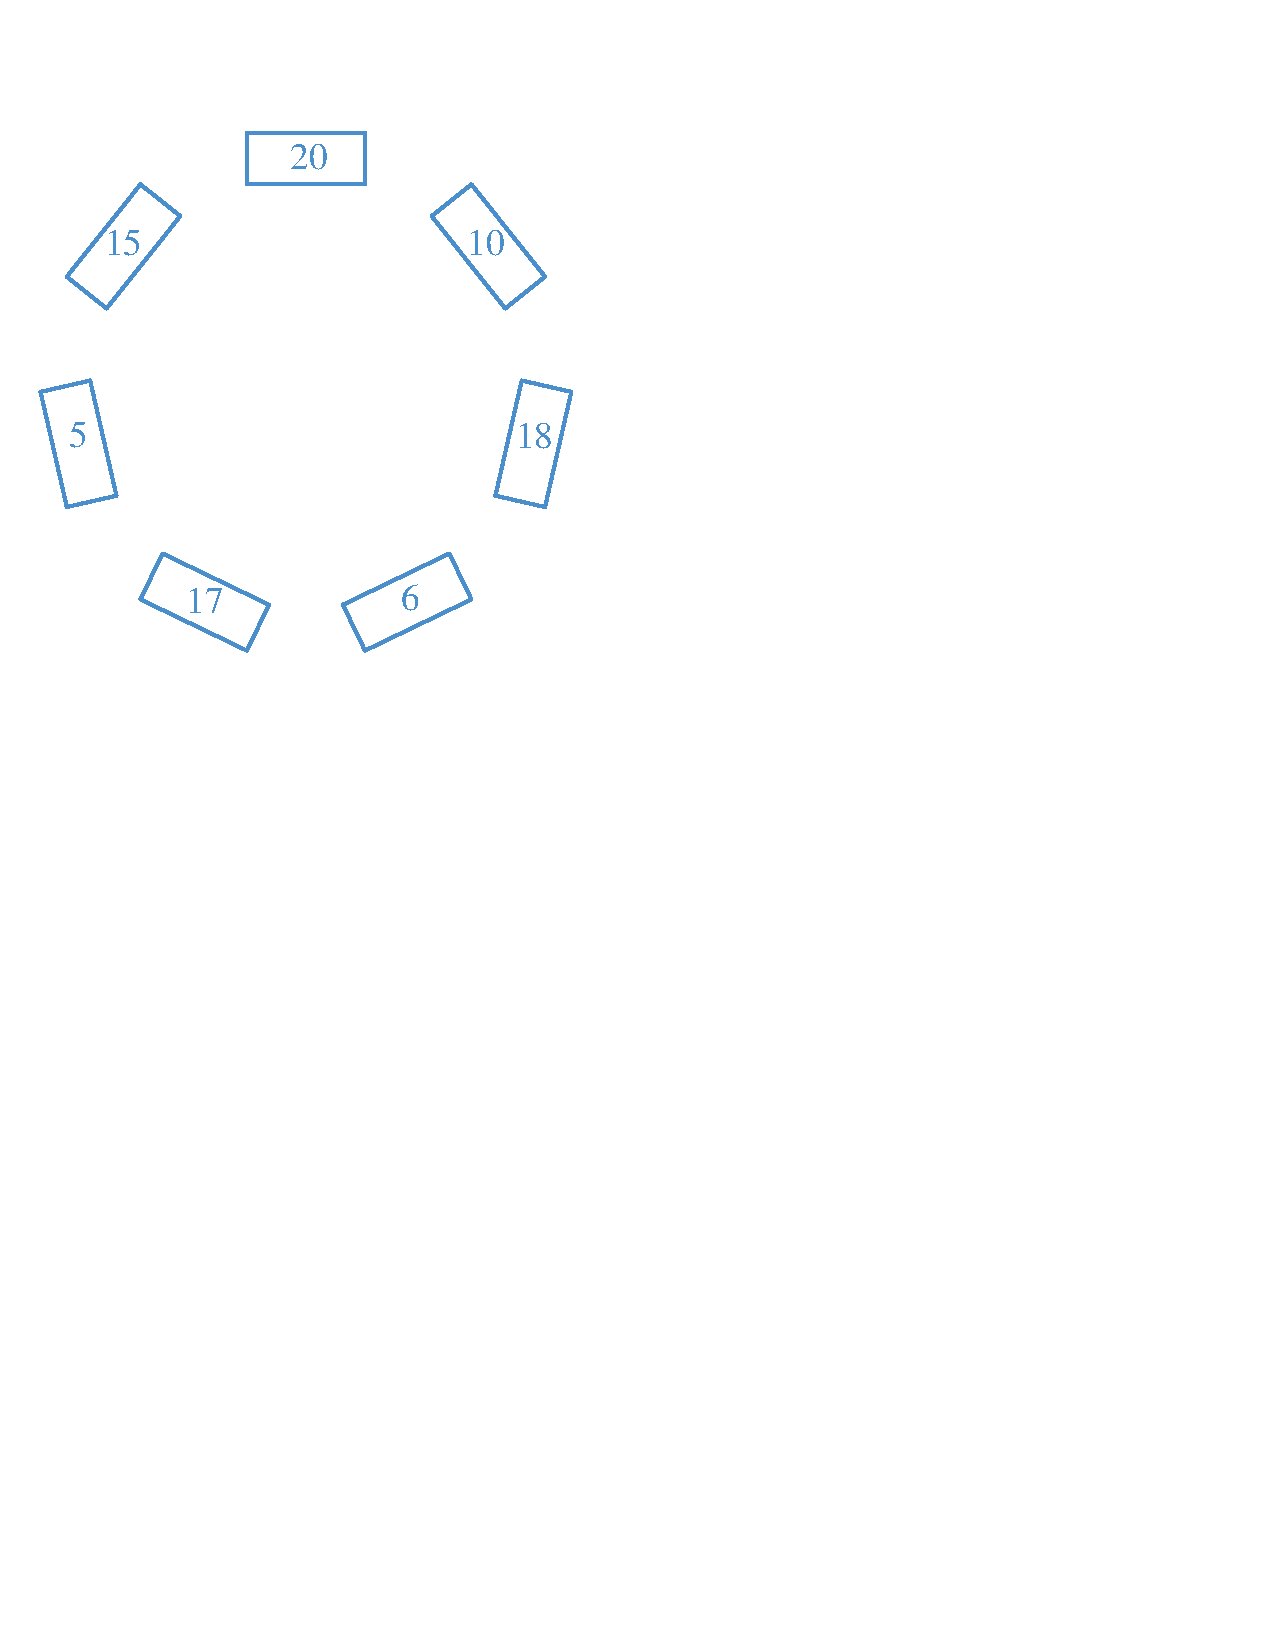
\includegraphics[width= 0.85\linewidth]{2.pdf}
		\vspace*{-5pt}
	\end{figure}
	\textit{Lời giải.}  Có tổng cộng $91$ đồng xu, do đó khi số đồng xu trong mỗi hộp bằng nhau thì mỗi hộp có đúng $13$ đồng xu. Như vậy những hộp ban đầu chứa lớn hơn $13$ đồng xu thì số đồng xu phải chuyển đi ít nhất bằng số chênh lệch so với $13$. Từ hộp chứa $20$ đồng xu, gọi là hộp $M,$ phải có ít nhất $\pmb{7}$ đồng chuyển đi. Xét hai hộp ở hai bên của hộp $M$, tổng số đồng xu trong $2$ hộp này ban đầu là $25$. Do có $7$ đồng xu từ hộp $M$ chuyển sang các hộp này, nên phải có ít nhất $25+ 7- 2\times 13= \pmb{6}$  đồng xu được chuyển đi từ hai hộp này.
	\vskip 0.1cm
	Cũng lý luận tương tự, từ các hộp chứa $17$ và $18$ đồng xu phải có lần lượt ít nhất là $\pmb{4}$ và $\pmb{5}$ đồng xu được chuyển đi. Như vậy, tổng số lần di chuyển không ít hơn $7+ 6 + 4 + 5 =22$.
	\vskip 0.1cm
	Ta có thể làm cho tất cả các hộp đều có $13$ đồng xu sau đúng $22$ lần di chuyển theo sơ đồ dưới đây. 
	\begin{figure}[H]
		\vspace*{-5pt}
		\centering
		\captionsetup{labelformat= empty, justification=centering}
		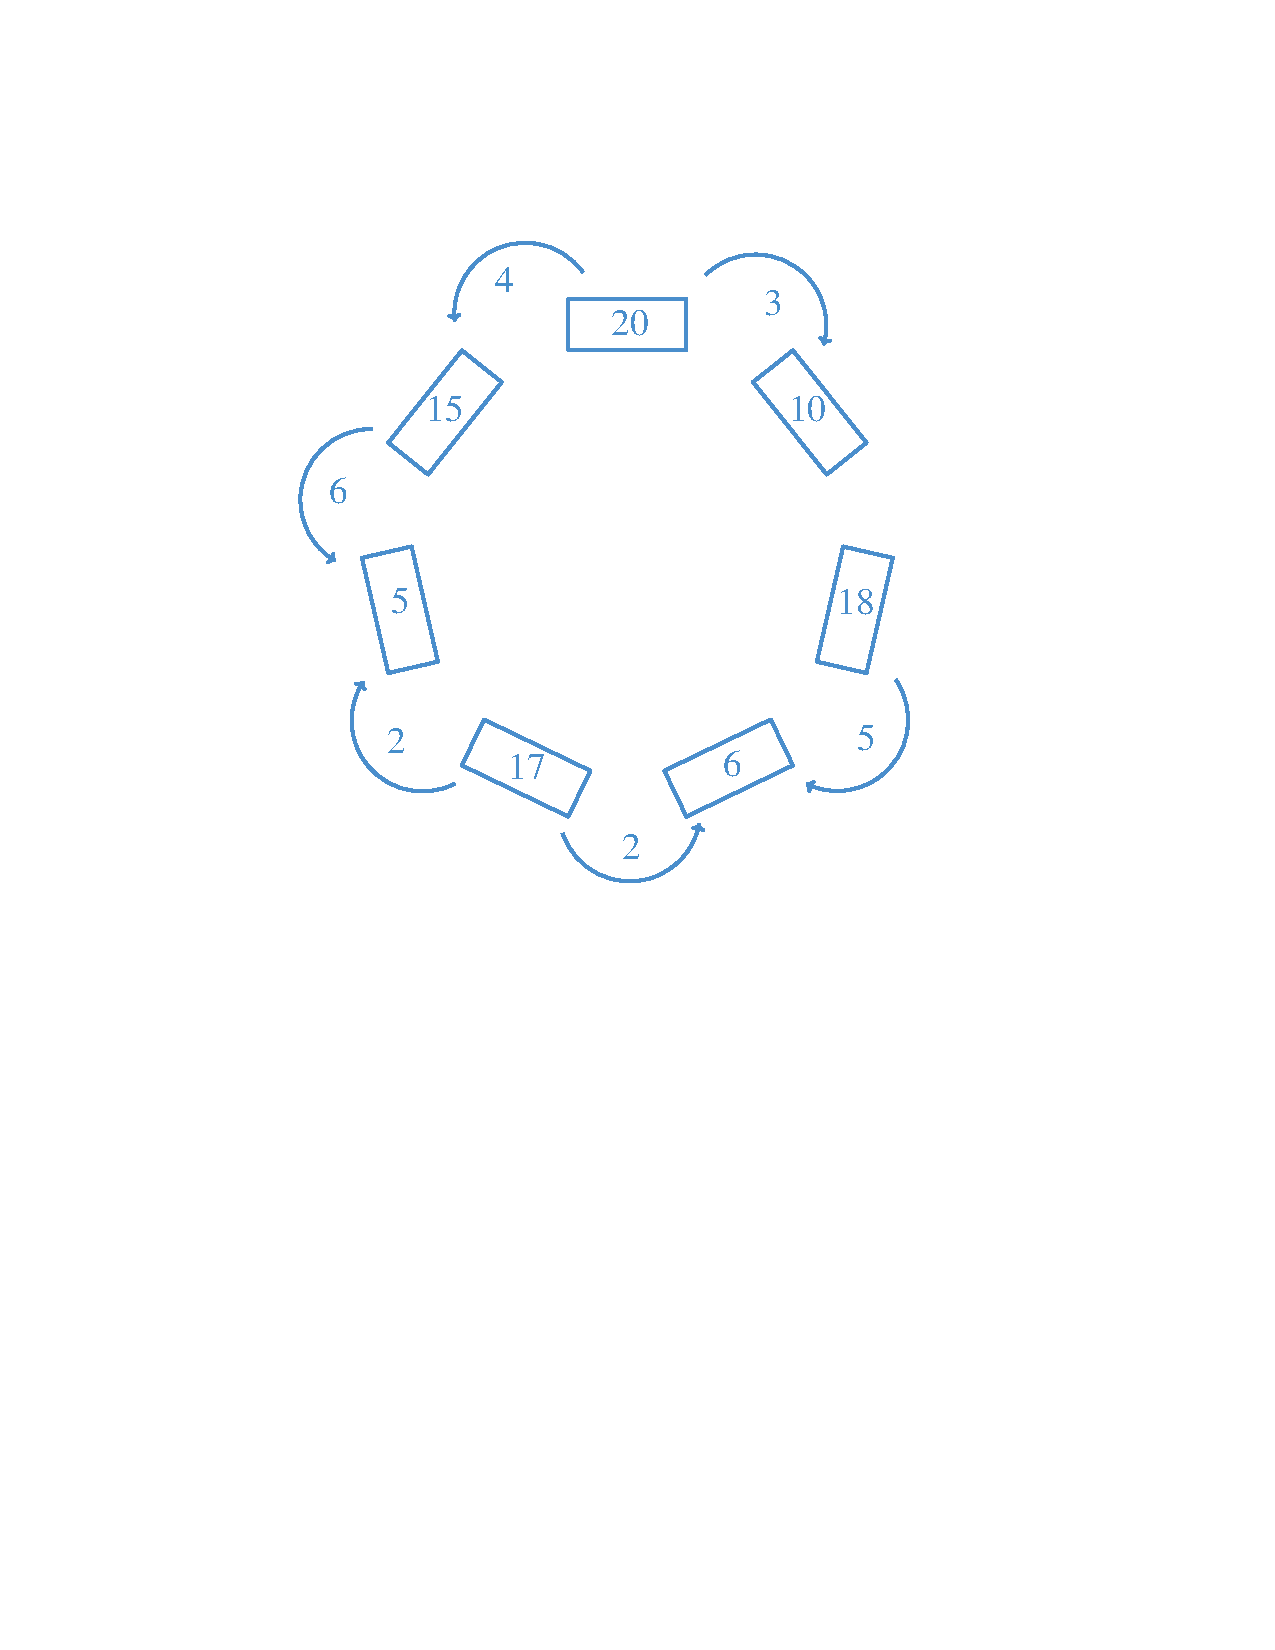
\includegraphics[width= 0.95\linewidth]{2a.pdf}
		\vspace*{-10pt}
	\end{figure}
	Trong phần cuối của chuyên mục kỳ này, chúng tôi sẽ giới thiệu với bạn đọc ba bài toán trong kỳ thi Olympic Toán thành phố Kiev (Ukraina), năm $2022$, dành cho khối lớp $7$. Lưu ý rằng hệ thống giáo dục phổ thông của Ukraina và Nga gồm $11$ lớp (từ lớp $1$ đến lớp $11$), do đó khối lớp $7$ của họ tương đương với khối lớp $8$ của Việt Nam.
	\vskip 0.1cm
	{\bf\color{cackithi} OC$\pmb{19.}$}  Viết phân số $\dfrac{1}{2021}$ thành hiệu của hai phân số tối giản có mẫu số nhỏ hơn.
	\vskip 0.1cm
	{\bf\color{cackithi} OC$\pmb{20.}$} Có $n$ tấm thẻ, trên đó viết lần lượt các số thực (không nhất thiết phân biệt): $a_1, a_2, \ldots, a_n$.  Xét tất cả $ (2^n-1) $ cách chọn ra một tập khác rỗng các tấm thẻ và tính tổng các số trên mỗi tập thẻ đã chọn. Hỏi trong số $(2^n-1)$ tổng nhận được có thể có nhiều nhất bao nhiêu số bằng $1$?
	\vskip 0.1cm
	Ví dụ: với $3$ tấm thẻ có số $-1, 2, 2$, thì các tổng thu được là $4, 3, 2, 2, 1, 1, -1.$ Do đó có hai tổng bằng $1$.
	\vskip 0.1cm
	{\bf\color{cackithi} OC$\pmb{21.}$} Trong tam giác $ ABC,$ đường trung tuyến $BM $ bằng một nửa cạnh $ BC $. Chứng minh rằng $ \angle ABM = \angle BCA + \angle BAC .$
\end{multicols}